\documentclass[conference,10pt,letterpaper]{IEEEtran}
\usepackage[T1]{fontenc}
\usepackage[utf8]{inputenc}
\usepackage{graphicx,booktabs,amsmath,url}
\usepackage[hidelinks]{hyperref}
\urlstyle{same}
\renewcommand{\ttdefault}{lmtt}
\graphicspath{{figures/}}
\hypersetup{pdftitle={From Public Data to Prediction Benchmarks: Cost, Reliability, and Lessons from an Agent-Driven Factory},pdfauthor={Eduardo Arino de la Rubia}}
\title{From Public Data to Prediction Benchmarks:\\Cost, Reliability, and Lessons from an Agent-Driven Factory}
\author{\IEEEauthorblockN{Eduardo Ari\~no de la Rubia}\IEEEauthorblockA{Central European University\\\texttt{rubiae@ceu.edu}}}
\begin{document}
\bstctlcite{IEEEexample:BSTcontrol}
\maketitle
\begin{abstract}
An agent-driven Dataset Factory published 11 prediction datasets on GitHub and Hugging Face during an interim 64.9-hour observation window. Estimated recurring operating cost was \$27.84--\$27.94, or \$2.53--\$2.54 per publication, including unsuccessful production work, workers, and allocated hosting. The factory connects public-source discovery, prediction-task construction, validation, and versioned publication. A deterministic controller manages state, workers, retries, and transfer; bounded language-model tasks interpret sources, generate code, and review meaning. This is an operating-window ratio, not a human-cost comparison or a development-cost estimate. Independent consumers completed three XGBoost research attempts on each of seven releases; four other releases encountered provider-access or quota failures. Saved results show modeling headroom on some tasks, but source review also identifies population-selection discrepancies, missing dependence keys, and a history feature whose safe use depends on the scoring interface. We describe the engineering and evaluation boundaries that make these outcomes inspectable. The experience supports low recurring cost for an integrated factory, while showing why public delivery, predictive performance, and benchmark validity require separate evidence.
\end{abstract}
\begin{IEEEkeywords}agentic engineering, dataset construction, prediction benchmarks, operating cost, empirical evaluation\end{IEEEkeywords}

\section{Introduction}
Dataset Factory connects public-source discovery to prediction-benchmark publication. In 64.9 hours it released 11 datasets across courts, utilities, safety regulation, research funding, transport, and environmental reporting. Independent consumers tested seven releases. This experience lets us examine recurring cost and product quality together.

Preparing a prediction benchmark requires more than downloading a table. Someone must find a source, interpret its records, define an observable outcome, identify available inputs, construct splits, check the result, and distribute an artifact that another researcher can use. Analyst interviews and repository curation records document substantial work in discovery, transformation, and quality checks~\cite{kandel,lafia}. The resulting software and data depend on executable transformations, contracts, tests, and versioned state. A boundary failure can invalidate otherwise successful work.

Recent systems already automate important parts of this process. AutoData collects web records from a natural-language request~\cite{autodata-web}; DatasetResearch evaluates demand-driven discovery~\cite{datasetresearch}; MLE-Smith constructs machine-learning tasks from supplied datasets~\cite{qiang2026mlesmith}; and AutoSDT searches sources and constructs executable scientific tasks~\cite{autosdt}. Low marginal generation cost is therefore not, by itself, a new result. Our interest is the operation of these capabilities as a continuing factory, including failed attempts, resource accounting, public delivery, and use by separate consumers.

We ask three questions. \textbf{RQ1:} What does a deployed factory produce, and which operational failures and interventions occur? \textbf{RQ2:} What recurring resources does that production consume? \textbf{RQ3:} What does independent use reveal about the published artifacts? The contribution is an experience report with inspectable records, not a new generation algorithm or a claim of first automation.

The system uses DeepSeek for production and Fable for independent evaluation. A standing policy permits publication without per-dataset human approval. People developed the system, set policy, and directed repairs; operation was not intervention-free.

\textit{Draft scope.} This draft uses the production export ending 15 November 2026 at 14:24 UTC and the original consumer results available at that point. Collection and three quota-recovery evaluations remain active. The paper will replace this interim snapshot with the final observation record before submission; no recovery result is assumed here.

\section{System and Work Allocation}
\subsection{The product and its boundaries}
Each release defines a binary prediction task from real public records. It includes a target, population, predictor contract, chronological split definition, baseline, source and license evidence, construction code, dependencies, and checksummed data. GitHub carries versioned release assets and code; Hugging Face carries the accepted files and a dataset card. The factory's code is public.\footnote{\url{https://github.com/earino/dataset-factory}}

The task contract distinguishes retrospective research from historical forecasting. A current administrative snapshot can support retrospective comparisons while failing to establish which fields were available at a past operational decision. The release must state that limitation. A narrower claim does not excuse incorrect labels, known answer exposure, or a population definition that contradicts the code.

\begin{figure*}[t]
\centering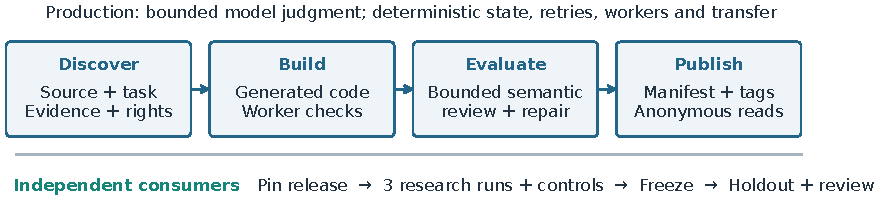
\includegraphics[width=\textwidth]{workflow.pdf}
\caption{Production and independent evaluation. Models handle source-specific judgment and code; deterministic software owns operational state and artifact movement. Consumer outcomes are not returned to production as optimization feedback during the observation window.}
\label{fig:workflow}
\end{figure*}

\subsection{Known procedures run in code}
A scheduled controller advances durable SQLite state through \emph{discover}, \emph{build}, \emph{evaluate}, and \emph{publish}. Saved attempts, responses, and artifact identities support resumption. Scout alone launches temporary Hetzner workers for downloads, transformations, fitting, and transfer. Independent cleanup handles expired workers.

Bounded model tasks interpret sources, propose prediction tasks, generate code, and review meaning. Repairs reuse proposals and diagnostics. Code checks transfer and worker state. The requested production model is \texttt{deepseek-v4.1-flash:1017}; records retain routing and usage.

Failures leave attempt records and diagnostics for reconciliation. Bounded retries and deferrals limit work on a source. An access error, a malformed response, and an unsuitable label remain distinct causes.

\subsection{Acceptance and publication}
Construction runs artifact checks on the worker. These include file and schema compatibility, labels, split consistency, task-specific leakage checks, and a working baseline. A bounded semantic review examines the evidence and the meaning of the constructed task. It can accept, request a material repair, or reject. Distribution requires readable source terms and preserved attribution.

A manifest binds accepted bytes. Publication transfers matching files to both platforms, tags the complete release, and verifies anonymous consumption. Frozen versions remain available; corrections must not silently replace evaluated data.

\section{Observation and Evaluation Method}
\subsection{Production record and cohort}
The prospective observation began on 12 November 2026 at 21:27:59 UTC. This draft ends its production accounting at 15 November at 14:24:01 UTC, covering 64.93 hours. The planned final cutoff is 16 November at 07:00 UTC. A read-only export contains candidate and attempt records, model usage, worker lifetimes, and publication identities. Periodic public snapshots provide an additional view, but do not replace the attempt ledger.

At the interim export, the ledger includes 42 candidate records created before the window and 65 admitted during it. Seven already-published dataset identities are excluded from the new consumer cohort. An admitted record is initially a search slot, not necessarily a distinct source. We count completed milestones by candidate and repeated work by attempt, rather than merge these denominators into one success rate.

Consumers select the first 12 new dataset identities by publication-verification time, breaking ties by identifier. Eleven had appeared at the interim cutoff; all eleven were new admissions. Selection does not depend on domain, baseline score, or consumer improvement. The first accepted version is pinned, and failures keep their place. Earlier pilot outcomes are not pooled with this cohort.

Discovery continues during consumer evaluation, without consumer feedback to selection or acceptance. Production repairs remain recorded interventions.

\subsection{Cost accounting}
We estimate recurring production cost as
\begin{equation}
 C_{\mathrm{window}}=C_{\mathrm{inference}}+C_{\mathrm{workers}}+C_{\mathrm{hosting}}.
\end{equation}
Inference uses recorded uncached input, cached input, and output tokens multiplied by dated published rates. Hermes reports those input categories separately; cached input is not added a second time to an inclusive total. Provider-specific peak and off-peak schedules are applied where timestamps permit. For sessions crossing a tariff boundary, the lower and higher applicable prices form a range. An all-peak alternative shows sensitivity to that allocation.

Ollama-routed usage is valued at Ollama rates. Earlier Nous-routed DeepSeek usage is valued at direct DeepSeek equivalents, not described as a Nous invoice. Recorded provider rates supply the worker estimate, including IPv4 and tax. Each server lifetime is rounded up separately to whole billed hours. Hosting is allocated from the author's \$20 monthly Nous plan over November's 30 days. The exchange rate used is \$1.1052 per euro. Rates and their retrieval date, 15 November, are retained with the calculation.

All recorded production work in the selected accounting window contributes, including unsuccessful attempts. Two model sessions and one worker crossing the starting boundary are included in full; other earlier work is excluded. Cost divided by publications is therefore a window-level operating ratio, not each artifact's lifetime construction cost. We separately retain candidate origin and publication timing.

The estimate excludes system development, author and operator labor, paper preparation, upstream agencies' data collection, and unmetered external services. The independent consumer experiment is a research instrument, covered by a separate Claude subscription, and is excluded from factory production costs. We have no matched human-construction experiment and report no labor savings ratio.

\subsection{Independent prediction experiments}
Each dataset receives three fresh Fable 5.2 research attempts, with an 85-minute allowance, three concurrent attempts, and five fitting threads each. One dataset is evaluated at a time. Requested and reported model identifiers are recorded. Prior repeated-run evidence shows variation between identical agent configurations and score inflation from protocol violations~\cite{identical-runs}. We therefore retain every attempt and examine conduct separately; three attempts describe variation, not a language-model ranking.

Consumers can change XGBoost~\cite{xgboost} preprocessing, feature transformations, and hyperparameters, using training and labeled validation data. The allowed raw predictor set comes from the pinned construction contract. Identifiers, carry columns, and label-source fields are excluded. An ordinary XGBoost scaffold and a per-attempt random-search control use the same permissible predictors. Random search follows the existing control procedure~\cite{randomsearch}; its budget matches recorded eligible fitting CPU, not total model-inference time or every exploratory diagnostic.

Selection uses replayed validation AUC, with ties resolved to the first trial. Selected code, fitted models, and validation predictions are frozen before holdout scoring. All attempts and controls for a dataset cross the freeze barrier before its holdout is fetched. Scoring uses the saved model and row-wise inference; the consumer cannot improve its model after seeing the result. Repeated validation optimization can still overfit selection~\cite{cawley}, which is why validation gains alone are not the result.

Holdouts are publicly available. Consumers are instructed not to access them, other runs, or coordinator files. The isolation is procedural, not an operating-system security boundary. Transcripts, tool requests, copied-file hashes, and selected code are retained for conduct review. An automatic access flag requires interpretation; its absence is not proof of compliance. Provider failures are recorded separately from dataset failure. After the author reset an exhausted quota, fresh recovery attempts were authorized for three affected datasets with the same release pins; those results are not included in this draft.

\subsection{Source review, uncertainty, and artifact probes}
A separate bounded review precedes scoring. It reads the task contract, construction code, source documentation, and permitted public data to examine target meaning, feature timing, population selection, and possible label-derived history. It also declares a dependence grouping from source meaning. The review does not approve publication or choose which datasets receive evaluation.

Where a grouping is available, paired bootstrap intervals resample whole groups 2,000 times, using a fixed seed derived from the dataset identifier. Each draw applies the same sampled rows to the consumer and control. Intervals are pointwise percentile 95\% intervals conditional on the fitted models, observed cohort, and grouping assumption. They do not include variation across future agent runs, temporal shifts, or all residual dependence. No multiplicity adjustment is applied. We do not average these intervals into a population-wide agent success probability.

Derived probes inspect row-order behavior, batch-versus-single-row preparation, external activity during preparation, and dependence of a training row's encoded features on its own label. These are targeted checks, not universal proofs. Their execution status and per-run diagnostics are read separately. This draft retains raw scores where semantic review or a probe is unresolved; it does not silently turn them into protocol-qualified outcomes.

\section{Results}
\subsection{Production across sources}
The window contains 394 started stage attempts. Forty-one candidates completed discovery, 14 a build, and 11 acceptance and publication. Repeated stages matter: 27 successful builds belong to 14 candidates. These milestones are not a completed-cohort conversion rate; other candidates remained deferred, rejected, or active.

The eleven published tasks cover civil trials, utility reliability, pipeline-enforcement penalties, device recalls, airline-route persistence, research-grant progression, air-pollution enforcement, wastewater exceedances, aircraft wildlife strikes, building permits, and railway hazardous-material releases. For these successful releases only, elapsed time from candidate admission to verified publication ranged from 40 to 189 minutes, with a median of 106 minutes. This excludes unsuccessful candidates' waiting time and does not measure how long an arbitrary source will take.

The ledger records 76 discovery retries, 184 build retries, and 14 semantic repair outcomes (Fig.~\ref{fig:operations}). Retries can include waiting or reconciliation, so they are neither model-call counts nor unique defects.

\begin{figure*}[t]
\centering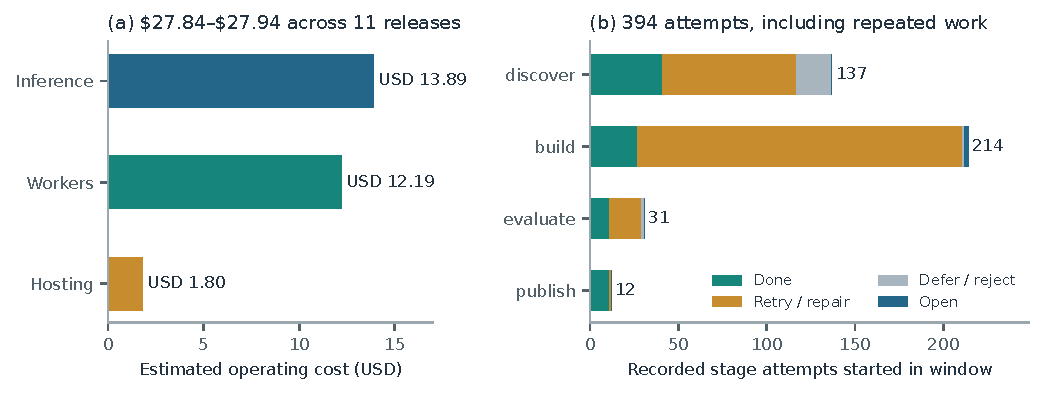
\includegraphics[width=\textwidth]{operations.pdf}
\caption{Interim production accounting, 12--15 November. (a) Estimated recurring cost; the inference bar uses the midpoint of the tariff-timing range. (b) Stage attempts started in the window, including repeated work. Counts are not unique sources or model calls.}
\label{fig:operations}
\end{figure*}

One documented intervention corrected worker-budget accounting on 14 November. The old admission calculation kept worst-case reservations after workers had been deleted, leaving almost no construction headroom. The shared code was changed to charge confirmed lifetimes in rounded hours while retaining reservations for active or unresolved records. The ordinary scheduler then resumed construction without manual candidate-state edits. The correction did not change the acceptance rules, but it affected the factory's ability to operate. It therefore belongs in the production account. A final reconciliation of all deployment and routing events remains part of the submission review; this draft makes no claim that this was the only intervention.

\subsection{Operating cost}
The selected production record contains 374 model sessions with usage and 2,412 API calls: 21.69 million uncached input tokens, 91.11 million cached input tokens, and 15.18 million output tokens. Five further attempts lack usage counters; Scout's readback identifies HTTP 402 failures before generation with zero tokens. We retain that explanation and its provenance rather than infer zero from missing values alone.

Time-priced inference is \$13.84--\$13.95. Workers contribute EUR 11.03, or \$12.19, and allocated hosting contributes \$1.80. Total estimated recurring cost is \$27.84--\$27.94, equivalent to \$2.53--\$2.54 per publication. Pricing all recorded inference at peak rates instead gives \$39.27 total, or \$3.57 per publication. Neither calculation includes the excluded development and human costs.

The 187 worker job lifetimes total 18.53 elapsed server-hours but 188 billed hours after per-lifetime rounding; one worker remained active. Fractional runtime understates this charge basis, while permanent worst-case reservations overstate settled use.

\subsection{Independent use and predictive comparisons}
All eleven released baselines and ordinary consumer scaffolds produced holdout scores. Seven datasets also completed all three consumer research attempts, yielding 21 frozen consumer models. The other 12 original attempts failed at the CLI/provider layer: utility-reliability attempts encountered access failures, and the final three datasets encountered quota exhaustion. These are not observations that the datasets lack predictive value.

Table~\ref{tab:scores} reports the raw saved-model results, retaining all attempts rather than selecting the best run for the paper. The seven completed datasets span small and large holdouts and different dependence structures. Ordinary-scaffold AUC ranges from 0.557 for pipeline penalties to 0.893 for wastewater. Scores alone do not establish useful decision support, and the comparisons below remain conditional on the unresolved review items.

\begin{table*}[t]
\caption{Interim raw holdout AUC. Consumer and random columns show the range across three attempts, not confidence intervals. Groups are the prescoring dependence keys used for intervals. ``?'' means unresolved grouping; ``--'' means no completed consumer comparison. Review limitations apply, including two unresolved training-feature probes.}
\label{tab:scores}\centering\small
\begin{tabular}{lrrrrr}\toprule
Task & Holdout rows & Ordinary & Consumer range & Random range & Groups\\\midrule
\csname @@input\endcsname generated/score-rows.tex
\bottomrule\end{tabular}
\end{table*}

Under district resampling, all three civil-trial comparisons against their random controls have positive intervals. Device-recall comparisons also have positive intervals under product-code resampling, but that key does not cover all dependence between firms or recall events. The civil-trial review also identifies defendant jury-demand information that can postdate filing. These comparisons establish headroom on the shipped retrospective tables, not valid prediction at filing or clearance time.

The remaining results are less decisive. All three air-enforcement point differences against random search are positive, but their intervals include zero. All three research-grant differences are negative with intervals including zero. Airline-route differences change sign across attempts, and every interval includes zero. For wastewater, one of three intervals is narrowly above zero and two include zero. We do not turn that isolated result into a general superiority claim. Figure~\ref{fig:intervals} shows all available paired comparisons with random search.

For pipeline-enforcement penalties, the release omits the operator identifier needed to represent the main dependence described by its own documentation. The prescoring reviewer therefore left the grouping unresolved. Its positive point differences are descriptive only. Substituting independent-row intervals would answer a different question without resolving the missing information.

\begin{figure*}[t]
\centering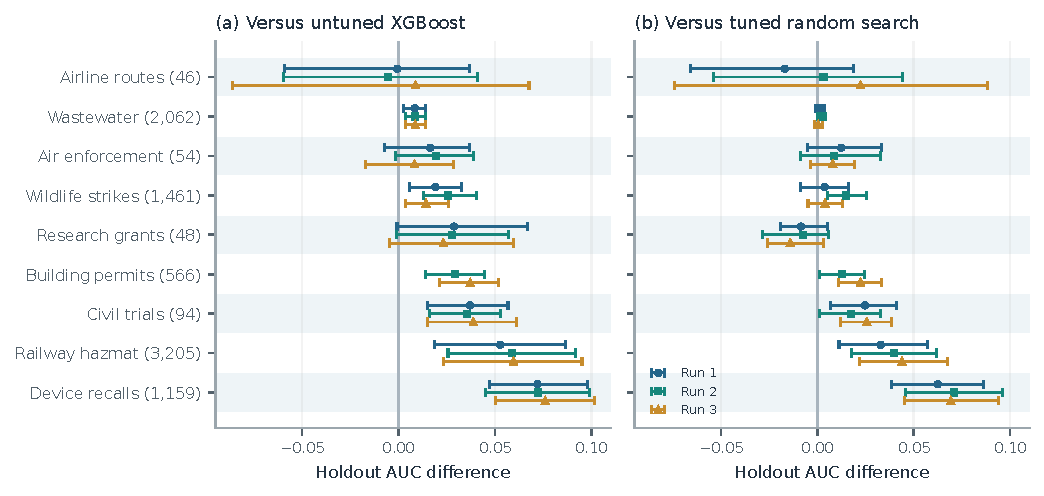
\includegraphics[width=\textwidth]{consumer-intervals.pdf}
\caption{Consumer minus paired random-search holdout AUC, with 2,000-draw whole-group percentile 95\% intervals. Every available attempt is shown. The FDA product-code grouping is partial; PHMSA operator grouping is unavailable and is omitted. These raw comparisons are conditional on fitted models and review limitations, not a ranking of consumer agents.}
\label{fig:intervals}
\end{figure*}

\subsection{What the score does not check}
The source and artifact reviews provide three concrete lessons beyond score differences.

\textbf{Selection logic can contradict the declared population.} In the SBIR research-grant task, eligibility depends on all records for a firm, including records after the index award. The code excludes firms with Phase I and Phase II in the same first year and uses ambiguity sets populated from later records. The contract nevertheless says that no outcome field is used to select rows. We confirmed these paths in the pinned builder and declaration. This is a documentation/selection discrepancy; the effect size is not established here. A separate suspicion that award amounts contain later options remains a hypothesis, not a proven leakage mechanism.

\textbf{A history feature needs an access contract.} The wastewater release uses the previous year's exceedance as a predictor for the current year. The prescoring review found exact agreement with the earlier row's label on 11,800 available public row pairs. The pinned code confirms the lag construction. Such history can be legitimate when the earlier outcome is available. It also means that later rows can reveal earlier outcomes if an evaluator exposes the entire future feature matrix at once. Our scorer supplies one row at a time, and the three saved consumer preparations passed the sampled batch/order probes. This supports the tested interface, not unrestricted batch use or a universal absence of cross-row exposure.

\textbf{Completing a check is not passing it.} All 21 saved consumer preparations passed batch-versus-single-row and reverse-order probes on 25 validation rows. Own-label feature probes produced no changed tested cells in 19 runs, but returned an assertion error for one device-recall and one airline-route run. The wrapper recorded successful execution of the script; its per-run report preserved the unresolved errors. Neither an error nor a green wrapper proves leakage or compliance. The two cases require semantic follow-up before a final protocol-qualified interpretation.

\section{Discussion and Engineering Lessons}
\subsection{Integration is the relevant unit of experience}
The factory's contribution is repeated operation across boundaries: discovery, construction, recovery, and public delivery. A production-agent study identifies reliability as a central deployment challenge and reports a preference for controllable designs~\cite{production}. Our accounting repair and retained failure records illustrate that concern in dataset production. Deterministic state, saved proposals, and version-bound artifacts make failures inspectable; we did not isolate their effects through an architecture ablation.

\subsection{Affordability has a clear but limited meaning}
A few dollars per publication makes recurring experimentation plausible for a group that already has the system. The estimate exposes the effects of retries, billing granularity, and caching. It does not measure development or the work needed to verify a new domain's assumptions.

Analyst interviews describe discovery, wrangling, profiling, modeling, and reporting~\cite{kandel}. Repository logs record transformation and quality-assurance work~\cite{lafia}. These are useful analogues for the factory's connected tasks, but their products and responsibilities differ from ours; they supply no matched human-cost denominator. Chaining theory provides an interpretation of adjacent task automation~\cite{chaining}, not a causal explanation tested here. Policy, engineering, and responsibility for claims remain human work whose displacement we have not measured.

\subsection{Evaluate products at several levels}
Checksums establish identity, source review examines meaning, and frozen-model experiments test use. The findings suggest concrete changes: retain non-predictor dependence keys, specify information visible at scoring, and compare population declarations with selection code. These address observed defects without making every release pass a universal review cascade.

\section{Related Work}
\subsection{Discovery, construction, and operating cost}
AutoData collects web data from a request~\cite{autodata-web}, and DatasetResearch evaluates demand-driven discovery~\cite{datasetresearch}. MLE-Smith constructs competition-style tasks from supplied datasets~\cite{qiang2026mlesmith}; AutoSDT searches sources and generates executable scientific tasks~\cite{autosdt}. Thus source search and automated task construction both have precedents. DataMaster~\cite{datamaster} and agentic data engineering for model specialization~\cite{dataengineering} use downstream feedback to guide data work. Our contribution is a deployed source-to-publication workflow with independent consumers, rather than a claim to have invented its component capabilities.

Reported costs have different boundaries. AutoData's preparation-time comparison ends when collection begins. MLE-Smith's first arXiv version reports \$0.78 per task, including generation and verification; its architecture ablation reports different costs on a smaller sample. AutoSDT reports approximately \$0.55 per generated task. Our ratio includes recorded failed production work, workers, and hosting for public releases. These figures establish low-cost precedents, not an efficiency ranking.

\subsection{Artifact quality and independent use}
AutoDataBench evaluates generated executable tasks for validity, novelty, difficulty, and behavioral coverage~\cite{autodatabench}. CurationBench tests data-selection policies under a fixed training and evaluation recipe~\cite{curation}. Both make downstream artifact quality central; our source-contract review and separate consumers extend that concern to public prediction releases from an operating factory. Documentation practices likewise motivate explicit provenance, intended use, and limitations~\cite{datasheets}.

MLAgentBench and MLE-bench evaluate agents on machine-learning work~\cite{mlagentbench,mlebench}. Here, consumer agents evaluate products of a separate producer. Repeated-run and compliance findings~\cite{identical-runs} motivate reporting every attempt, while cost-aware agent evaluation~\cite{agents-matter} and random search~\cite{randomsearch} motivate controls. Model-selection bias~\cite{cawley} motivates freezing validation-selected models before holdout scoring. None of these controls replaces source-level checks of targets, populations, or available inputs.

\section{Threats to Validity and Evidence Availability}
This is one factory, a short observation period, one production-model family, one consumer configuration, and a small publication cohort. The interim record cannot estimate a general probability that a source becomes a useful benchmark. Continued operation and recovery evaluations may change the counts.

All tasks draw on existing public records. Packaging does not establish that the models have never seen these data. Public holdouts enable reproducibility and conduct testing, but procedural isolation cannot prove non-access. Transcript screening and sampled code probes have incomplete coverage. Semantic review of selected solutions and flagged requests remains incomplete.

Dependence keys are imperfect. Product-code grouping does not necessarily capture FDA firm and recall-event dependence; state grouping need not capture all environmental dependence; no suitable PHMSA operator key is shipped. Bootstrap intervals are conditional on these choices. Intervals cannot validate target, population, or input-timing claims.

Costs use measured resources and published rates, not reconciled invoices, with the exclusions in Section III. Release latency excludes deferred work. Routing and accounting changes prevent interpreting the window as a fixed-configuration benchmark.

The evidence repository retains release pins, attempts, models, predictions, transcripts, reviews, and analysis code. It is private during drafting and planned for public release at submission.\footnote{Planned evidence repository: \url{https://github.com/earino/factory-prospective-study}.} Replay of frozen artifacts is distinct from reproducing a fresh nondeterministic agent trajectory.

\section{Conclusion}
An agent-driven factory connected public-source discovery to versioned publication for 11 prediction datasets at an interim estimated recurring cost of about \$28. Independent consumers completed research on seven releases and exposed both modeling headroom and concrete limits in task specification and evaluation. The low operating cost is encouraging; it does not certify the products. Retaining evidence for source meaning, construction, recovery, cost, publication, and independent use makes inexpensive automation assessable.

\section*{AI Assistance}
AI systems assisted implementation, literature search, review briefs, source and transcript review, analysis, and manuscript drafting. Production and consumer models are identified in the method. The author retains responsibility for the claims, source verification, and final submitted text.

\bibliographystyle{IEEEtran}
\bibliography{refs}
\end{document}
